\documentclass{article}
\usepackage[utf8]{inputenc}
\usepackage[english]{babel}
\usepackage{amsmath}
\usepackage{graphicx}
\usepackage{subcaption}
\usepackage{array}
\usepackage{color}
\usepackage{float}
\usepackage{listings}
\usepackage{indentfirst}
\usepackage{csquotes}
\usepackage[pages=some]{background}
\usepackage{hyperref}
\usepackage{setspace}
\onehalfspacing
%\usepackage{parskip}
\usepackage{svg}
\usepackage{geometry}
\renewcommand{\baselinestretch}{1.15}
\usepackage{changepage}

\usepackage{tikz}

\setcounter{secnumdepth}{5}
\setcounter{tocdepth}{5}

\hypersetup{
    colorlinks=true,
    linkcolor=blue,
    filecolor=magenta,
    urlcolor=blue,
}

\newcommand*{\figref}[2][]{%
  \hyperref[{fig:#2}]{%
    Figure~\ref*{fig:#2}%
    \ifx\\#1\\%
    \else
      \,#1%
    \fi
  }%
}


\hypersetup{
    colorlinks=true,
    linkcolor=blue,
    filecolor=magenta,
    urlcolor=blue,
}

\lstset
{
    breaklines=true,
    breakatwhitespace=true,
    frame=single,
    columns=fullflexible,
    basicstyle=\ttfamily,
    showstringspaces=false,
    %numbers=left,
    %stepnumber=1,
    %numbersep=8pt,
}

\backgroundsetup{
scale=1,
color=black,
opacity=0.05,
angle=10,
position={12cm,-22cm},
contents={%
  \includegraphics[height=20cm,width=20cm,keepaspectratio]{sceau.jpg}
  }%
}

\begin{document}
\begin{titlepage}
    \begin{center}
        \BgThispage
        \vspace*{1cm}
        
        
        \huge
        \textbf{Visual Media Compression}
        \vspace{0.25cm}
        
        \LARGE
        \textbf{INFO-H516}
        
        \vspace{0.5cm}
        \LARGE
        {Exercises report}
        
        \vspace{3.5cm}
        
        \textbf{BAKKALI Yahya (000445166) \\}


        \vspace{2.5cm}
        \textit{May 2023 \\}
        \vspace{0.5cm}
        \textsc{Université Libre de Bruxelles (ULB)}
        
        
    \end{center}
\end{titlepage}

\tableofcontents
\thispagestyle{empty}
\newpage
\setcounter{page}{1}
\setlength{\parskip}{1em}

\section{Introduction}

The field of visual media compression plays a crucial role in various applications, ranging from multimedia streaming to efficient storage of large-scale visual data. In this report, we present the results and findings of the image and video compression exercises for the Visual Media Compression course. There are four tasks, each covering different aspects of compression techniques. Our first task was to implement an image encoder and decoder for image compression and decompression. The second and third tasks focused on video compression, where we designed a video encoder and decoder to efficiently compress and decompress video. In the second task we used only I-frames, while in the third task we extended the previous implementation by incorporating both I-frames and D-frames, with the aim of improving compression performance and reducing bitrate requirements. Finally, we compared the performance of the codecs implemented with existing compression standards: for image task, we used JPEG and JPEG2000, and for video tasks, H.264 and H.265.

\section{Task 1}
\subsection{Description}

In the first task of our report, we focused on simulating an image encoder and decoder. Our approach involved applying block-based coding, where we divided the image into blocks for efficient processing. We implemented the Discrete Cosine Transform (DCT) and Inverse DCT per block to convert the image data from the spatial domain to the frequency domain and vice versa. Quantization and inverse-quantization techniques were applied to reduce the precision of the frequency coefficients and subsequently reconstruct them. To optimize the encoding process, we implemented zigzag and inverse zigzag scan per block, which rearranged the coefficients in a specific order for better compression efficiency. Finally, we implemented entropy encoding/decoding to further reduce the data size by assigning shorter codes to more frequently occurring symbols.

\subsection{Encoder implementation}
\subsubsection{Block-based coding}

The first step was to divide the original image, with dimensions (W, H), into non-overlapping blocks of size (N, N). In our case, we have applied this step to the Lena image, whose dimensions are (256 , 256) and which has been divided into blocks of size (8 ,8).

To illustrate this process, the original Lena image was displayed alongside the split representation. The original image shows Lena in grayscale. In contrast, the split image of Lena contains a grid of blocks, with each block clearly delineated. Each block measured 8 by 8 pixels and contained a segment of Lena's image.

\begin{figure}[H]
  \centering
  \begin{subfigure}[b]{0.45\textwidth}
    \centering
    \includegraphics[width=\textwidth]{Project/images/lena.png}
    \caption{Lena image}
    \label{fig:image1}
  \end{subfigure}
  \hfill
  \begin{subfigure}[b]{0.45\textwidth}
    \centering
    \includegraphics[width=\textwidth]{Project/images/lena_blocks.png}
    \caption{Lena image blocks}
    \label{fig:image2}
  \end{subfigure}
  \caption{Split Lena image of size (256, 256) into blocks of size (8,8)}
  \label{fig:overall}
\end{figure}

\subsubsection{DCT}

After dividing the image into blocks, the next step in block-based coding is to apply the Discrete Cosine Transform (DCT) to each block. The DCT converts the spatial domain pixel values into frequency domain coefficients. The two-dimensional DCT of an image block is simply the one-dimensional DCT performed along the rows and then along the columns. For our project we implement DCT-II, the formulas that we used comes from scipy~\footnote{\url{https://docs.scipy.org/doc/scipy/reference/generated/scipy.fftpack.dct.html##scipy-fftpack-dct}} library.
For the one-dimensional DCT the formula is the following:  

\[
y_k = 2 \sum\limits_{n=0}^{N-1} x_n \cos\left(\frac{\pi k(2n+1)}{2N}\right) \qquad \text{for } k=0,\dots,N-1.
\]

Where N is the number of elements in the array. Then, to normalize the value of $y_k$, we multiply it by a scaling factor f as follows:

\[
f = \left\{
\begin{array}{ll}
\sqrt{\frac{1}{4N}} & \text{if}\ k = 0, \\
\sqrt{\frac{1}{2N}} & \text{otherwise}
\end{array}
\right.
\]

Let's consider an example using a block from the divided Lena image, where the block size is 8 by 8 pixels. We will calculate the DCT coefficients for the first block.

\begin{figure}[H]
  \centering
  \hspace*{-1.5cm}
  \begin{tabular}{ccc}
    \begin{tabular}{c}
       $\begin{bmatrix}
        137 & 136 & 133 & 136 & 138 & 134 & 134 & 132 \\
        137 & 136 & 133 & 136 & 138 & 134 & 134 & 132 \\
        138 & 133 & 134 & 134 & 136 & 132 & 130 & 130 \\
        133 & 133 & 133 & 130 & 134 & 133 & 128 & 125 \\
        129 & 133 & 130 & 130 & 133 & 131 & 132 & 128 \\
        131 & 133 & 130 & 122 & 132 & 131 & 130 & 130 \\
        131 & 130 & 130 & 130 & 132 & 131 & 128 & 130 \\
        131 & 132 & 130 & 130 & 131 & 131 & 130 & 128 \\
      \end{bmatrix}$
    \end{tabular}
    &
    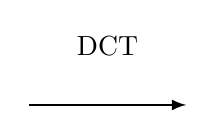
\begin{tikzpicture}[>=latex]
      \draw[->,thick] (0,0) -- (2,0);
      \node[above] at (1,0.5) {DCT};
    \end{tikzpicture}
    &
    \begin{tabular}{c}
       $\begin{bmatrix}
        1056 & 7 & -3 & 7 & 0 & -4 & -2 & 3 \\
        15 & 3 & -2 & 1 & 4 & 2 & -2 & 0 \\
        6 & -1 & 1 & -1 & 3 & 2 & -1 & -2 \\
        -1 & -4 & 3 & 0 & -2 & -3 & -2 & 1 \\
        -1 & 0 & -3 & 0 & -2 & 1 & -2 & -1 \\
        -2 & 2 & -1 & 0 & 1 & 0 & 3 & 0 \\
        -1 & 1 & 3 & 1 & -1 & -1 & 1 & 2 \\
        1 & -1 & -1 & -2 & 3 & 2 & -1 & -1 \\
      \end{bmatrix}$      
    \end{tabular}
  \end{tabular}
  \caption{Example of DCT execution on the first block}
  \label{fig:dct}
\end{figure}

\subsubsection{Quantization}

Once the DCT coefficients have been calculated for each block, the next step in the encoding is quantization. Quantization reduces the precision of the DCT coefficients to achieve compression. The process involves dividing the DCT coefficients by a quantization matrix, which controls the level of compression and determines the amount of information discarded. The quantization matrix used for this project is the following:

\[
Q = \begin{bmatrix}
    16 & 11 & 10 & 16 & 24 & 40 & 51 & 61 \\
    12 & 12 & 14 & 19 & 26 & 58 & 60 & 55 \\
    14 & 13 & 16 & 24 & 40 & 57 & 69 & 56 \\
    14 & 17 & 22 & 29 & 51 & 87 & 80 & 62 \\
    18 & 22 & 37 & 56 & 68 & 109 & 103 & 77 \\
    24 & 35 & 55 & 64 & 81 & 104 & 113 & 92 \\
    49 & 64 & 78 & 87 & 103 & 121 & 120 & 101 \\
    72 & 92 & 95 & 98 & 112 & 100 & 103 & 99 \\
\end{bmatrix}
\]

Consider the first block of Lena's split image, which has been transformed using DCT. The DCT coefficients for this block have been obtained, and we will now apply quantization to this block. By dividing each DCT coefficient in the first block by the corresponding entry in the quantization matrix, we obtain the quantized DCT coefficients. The higher values in the quantization matrix result in greater loss of precision and hence more compression.

\begin{figure}[H]
  \centering
  \hspace*{-1.5cm}
  \begin{tabular}{ccc}
    \begin{tabular}{c}
       $\begin{bmatrix}
        1056 & 7 & -3 & 7 & 0 & -4 & -2 & 3 \\
        15 & 3 & -2 & 1 & 4 & 2 & -2 & 0 \\
        6 & -1 & 1 & -1 & 3 & 2 & -1 & -2 \\
        -1 & -4 & 3 & 0 & -2 & -3 & -2 & 1 \\
        -1 & 0 & -3 & 0 & -2 & 1 & -2 & -1 \\
        -2 & 2 & -1 & 0 & 1 & 0 & 3 & 0 \\
        -1 & 1 & 3 & 1 & -1 & -1 & 1 & 2 \\
        1 & -1 & -1 & -2 & 3 & 2 & -1 & -1 \\
      \end{bmatrix}$ 
    \end{tabular}
    &
    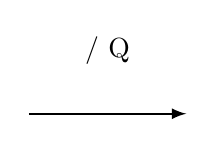
\begin{tikzpicture}[>=latex]
      \draw[->,thick] (0,0) -- (2,0);
      \node[above] at (1,0.5) {/ Q};
    \end{tikzpicture}
    &
    \begin{tabular}{c}
        $\begin{bmatrix}
          66 & 1 & 0 & 0 & 0 & 0 & 0 & 0 \\
          1 & 0 & 0 & 0 & 0 & 0 & 0 & 0 \\
          0 & 0 & 0 & 0 & 0 & 0 & 0 & 0 \\
          0 & 0 & 0 & 0 & 0 & 0 & 0 & 0 \\
          0 & 0 & 0 & 0 & 0 & 0 & 0 & 0 \\
          0 & 0 & 0 & 0 & 0 & 0 & 0 & 0 \\
          0 & 0 & 0 & 0 & 0 & 0 & 0 & 0 \\
          0 & 0 & 0 & 0 & 0 & 0 & 0 & 0 \\
        \end{bmatrix}$     
    \end{tabular}
  \end{tabular}
  \caption{Example of quantization execution on the first block}
  \label{fig:quantization}
\end{figure}

\subsubsection{Zigzag scan}

After quantization, the next step is the zigzag scanning. Zigzag scanning is performed on the quantized DCT coefficients of each block to rearrange them in a specific order, optimizing the compression efficiency. To illustrate the zigzag, we will use the quantized DCT coefficients of the first block of Lena's split image. \figref{zigzag} shows the original order of the quantized DCT coefficients and the zigzag scanning order to be followed.

\begin{figure}[H]
    \centering
    \includegraphics[width=0.5\textwidth]{Project/images/newplot.png}
    \caption{Zigzag scannig on the first block}
    \label{fig:zigzag}
\end{figure}

The resulting zigzag scanning order of quantized DCT coefficients is as follows:

\[
\begin{bmatrix}
  66 & 1 & 1 & EOB
\end{bmatrix}
\]

As the result shows, all trailing zeros are removed and the $EOB$ delimiter is inserted to separate the blocks. The $EOB$ will be used by the decoder to reconstruct the original block. For technical reasons, we replace the $EOB$ with $inf$ in our implementation.

\subsubsection{Entropy coding}

After the zigzag scanning stage, the next step is entropy coding. For this project, we used Huffman coding, a widely used entropy coding technique that assigns variable-length codes to symbols according to their probability of occurrence.  We apply Huffman entropy coding to the zigzag scanned quantized DCT coefficients of each block. By applying Huffman's entropy coding to the previous result of the first block, we obtain the following result:

\begin{figure}[H]
  \centering
  \hspace*{-1.5cm}
  \begin{tabular}{ccc}
    \begin{tabular}{c}
       $\begin{bmatrix}
          66 & 1 & 1 & EOB
        \end{bmatrix}$
    \end{tabular}
    &
    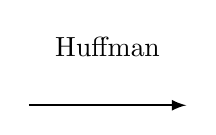
\begin{tikzpicture}[>=latex]
      \draw[->,thick] (0,0) -- (2,0);
      \node[above] at (1,0.5) {Huffman};
    \end{tikzpicture}
    &
    \begin{tabular}{c}
        b`\textbackslash xcb\textbackslash xe4'
    \end{tabular}
  \end{tabular}
  \caption{Example of Huffman encoding on the first block}
  \label{fig:entropy}
\end{figure}

\subsection{Decoder implementation}
\subsubsection{Entropy decoding}

Entropy decoding is the process of converting the variable-length Huffman codes back into the corresponding zigzag scanned quantized DCT coefficients. By using the Huffman codebook, which contains the mapping between codes and coefficients, the compressed data is decoded to obtain the original blocks.

\subsubsection{Inverse zigzag scan}

By applying inverse zigzag scanning, the coefficients are placed back into their respective positions within the block, recreating the original quantized DCT coefficients.

\subsubsection{Inverse quantization}

Both previous steps are lossless, however,    b   the inverse quantization is a lossy one. Inverse quantization aims to restore the quantized coefficients to their original values by multiplying them with the corresponding entries from the quantization matrix used during compression.

Let's use the example block we coded in the section above. Once we have applied entropy decoding and zigzag scanning, we get the same original block. We now perform inverse quantization on this block.

\begin{figure}[H]
  \centering
  \hspace*{-1.5cm}
  \begin{tabular}{ccc}
    \begin{tabular}{c}
        $\begin{bmatrix}
          66 & 1 & 0 & 0 & 0 & 0 & 0 & 0 \\
          1 & 0 & 0 & 0 & 0 & 0 & 0 & 0 \\
          0 & 0 & 0 & 0 & 0 & 0 & 0 & 0 \\
          0 & 0 & 0 & 0 & 0 & 0 & 0 & 0 \\
          0 & 0 & 0 & 0 & 0 & 0 & 0 & 0 \\
          0 & 0 & 0 & 0 & 0 & 0 & 0 & 0 \\
          0 & 0 & 0 & 0 & 0 & 0 & 0 & 0 \\
          0 & 0 & 0 & 0 & 0 & 0 & 0 & 0 \\
        \end{bmatrix}$  
    \end{tabular}
    &
    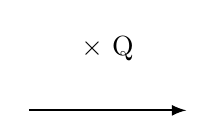
\begin{tikzpicture}[>=latex]
      \draw[->,thick] (0,0) -- (2,0);
      \node[above] at (1,0.5) {$\times$ Q};
    \end{tikzpicture}
    &
    \begin{tabular}{c}
        $\begin{bmatrix}
          1056 & 11 & 0 & 0 & 0 & 0 & 0 & 0 \\
          12 & 0 & 0 & 0 & 0 & 0 & 0 & 0 \\
          0 & 0 & 0 & 0 & 0 & 0 & 0 & 0 \\
          0 & 0 & 0 & 0 & 0 & 0 & 0 & 0 \\
          0 & 0 & 0 & 0 & 0 & 0 & 0 & 0 \\
          0 & 0 & 0 & 0 & 0 & 0 & 0 & 0 \\
          0 & 0 & 0 & 0 & 0 & 0 & 0 & 0 \\
          0 & 0 & 0 & 0 & 0 & 0 & 0 & 0 \\
        \end{bmatrix}$     
    \end{tabular}
  \end{tabular}
  \caption{Example of inverse quantization execution on the first block}
  \label{fig:iquantization}
\end{figure}

\figref{diffquantization} shows the difference between the original DCT coefficient for the first block and that obtained by inverse quantization. We can clearly see that this is a lossy step, as most of the values could not be restored.

\begin{figure}[H]
  \centering
  \hspace*{-1.5cm}
  \begin{tabular}{ccc}
    \begin{tabular}{c}
       $\begin{bmatrix}
        1056 & 7 & -3 & 7 & 0 & -4 & -2 & 3 \\
        15 & 3 & -2 & 1 & 4 & 2 & -2 & 0 \\
        6 & -1 & 1 & -1 & 3 & 2 & -1 & -2 \\
        -1 & -4 & 3 & 0 & -2 & -3 & -2 & 1 \\
        -1 & 0 & -3 & 0 & -2 & 1 & -2 & -1 \\
        -2 & 2 & -1 & 0 & 1 & 0 & 3 & 0 \\
        -1 & 1 & 3 & 1 & -1 & -1 & 1 & 2 \\
        1 & -1 & -1 & -2 & 3 & 2 & -1 & -1 \\
      \end{bmatrix}$ 
    \end{tabular}
    &
    $\neq$
    &
    \begin{tabular}{c}
        $\begin{bmatrix}
          1056 & 11 & 0 & 0 & 0 & 0 & 0 & 0 \\
          12 & 0 & 0 & 0 & 0 & 0 & 0 & 0 \\
          0 & 0 & 0 & 0 & 0 & 0 & 0 & 0 \\
          0 & 0 & 0 & 0 & 0 & 0 & 0 & 0 \\
          0 & 0 & 0 & 0 & 0 & 0 & 0 & 0 \\
          0 & 0 & 0 & 0 & 0 & 0 & 0 & 0 \\
          0 & 0 & 0 & 0 & 0 & 0 & 0 & 0 \\
          0 & 0 & 0 & 0 & 0 & 0 & 0 & 0 \\
        \end{bmatrix}$        
    \end{tabular}
  \end{tabular}
  \caption{Difference between original DCT coefficients (left) and the decoded (right) for first block}
  \label{fig:diffquantization}
\end{figure}


\subsubsection{Inverse DCT}

After inverse quantization, the decoder performed inverse DCT. The inverse DCT converts the frequency domain coefficients back into the spatial domain pixel values, reconstructing the image block as close as possible to the original. For the one-dimensional inverse DCT the formula is the following:  

\[
y_k = x_0 + 2 \sum_{n=1}^{N-1} x_n \cos \left(\frac{\pi (2k + 1)n}{2N}\right) \qquad \text{for } k=0,\dots,N-1.
\]

Where N is the number of elements in the array. For the inverse DCT of normalized values, this formula is used instead:

\[
y_k = \frac{x_0}{\sqrt{N}} + \sqrt{\frac{2}{N}} \sum_{n=1}^{N-1} x_n \cos\left(\frac{\pi (2k + 1)n}{2N}\right) \text{for } k=0,\dots,N-1.
\]

By applying the inverse DCT on the decoded first block we obtained the results below:

\begin{figure}[H]
  \centering
  \hspace*{-1.5cm}
  \begin{tabular}{ccc}
    \begin{tabular}{c}
        $\begin{bmatrix}
          1056 & 11 & 0 & 0 & 0 & 0 & 0 & 0 \\
          12 & 0 & 0 & 0 & 0 & 0 & 0 & 0 \\
          0 & 0 & 0 & 0 & 0 & 0 & 0 & 0 \\
          0 & 0 & 0 & 0 & 0 & 0 & 0 & 0 \\
          0 & 0 & 0 & 0 & 0 & 0 & 0 & 0 \\
          0 & 0 & 0 & 0 & 0 & 0 & 0 & 0 \\
          0 & 0 & 0 & 0 & 0 & 0 & 0 & 0 \\
          0 & 0 & 0 & 0 & 0 & 0 & 0 & 0 \\
        \end{bmatrix}$ 
    \end{tabular}
    &
    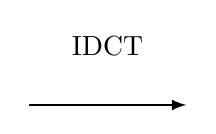
\begin{tikzpicture}[>=latex]
      \draw[->,thick] (0,0) -- (2,0);
      \node[above] at (1,0.5) {IDCT};
    \end{tikzpicture}
    &
    \begin{tabular}{c}
        $\begin{bmatrix}
          136 & 136 & 135 & 134 & 134 & 133 & 132 & 132 \\
          136 & 135 & 135 & 134 & 133 & 133 & 132 & 132 \\
          135 & 135 & 134 & 134 & 133 & 132 & 132 & 131 \\
          134 & 134 & 133 & 133 & 132 & 131 & 131 & 131 \\
          133 & 133 & 133 & 132 & 131 & 131 & 130 & 130 \\
          133 & 132 & 132 & 131 & 130 & 130 & 129 & 129 \\
          132 & 132 & 131 & 131 & 130 & 129 & 129 & 128 \\
          132 & 132 & 131 & 130 & 130 & 129 & 128 & 128 \\
        \end{bmatrix}$   
    \end{tabular}
  \end{tabular}
  \caption{Example of inverse DCT execution on the first block}
  \label{fig:idct}
\end{figure}

\figref{diffblock} shows the difference between the original the first block and that obtained by decoder. We can see that the values of the decoded are close to the original one even there was some data losses with quantization.

\begin{figure}[H]
  \centering
  \hspace*{-1.5cm}
  \begin{tabular}{ccc}
    \begin{tabular}{c}
       $\begin{bmatrix}
        137 & 136 & 133 & 136 & 138 & 134 & 134 & 132 \\
        137 & 136 & 133 & 136 & 138 & 134 & 134 & 132 \\
        138 & 133 & 134 & 134 & 136 & 132 & 130 & 130 \\
        133 & 133 & 133 & 130 & 134 & 133 & 128 & 125 \\
        129 & 133 & 130 & 130 & 133 & 131 & 132 & 128 \\
        131 & 133 & 130 & 122 & 132 & 131 & 130 & 130 \\
        131 & 130 & 130 & 130 & 132 & 131 & 128 & 130 \\
        131 & 132 & 130 & 130 & 131 & 131 & 130 & 128 \\
      \end{bmatrix}$
    \end{tabular}
    &
    $\neq$
    &
    \begin{tabular}{c}
        $\begin{bmatrix}
          136 & 136 & 135 & 134 & 134 & 133 & 132 & 132 \\
          136 & 135 & 135 & 134 & 133 & 133 & 132 & 132 \\
          135 & 135 & 134 & 134 & 133 & 132 & 132 & 131 \\
          134 & 134 & 133 & 133 & 132 & 131 & 131 & 131 \\
          133 & 133 & 133 & 132 & 131 & 131 & 130 & 130 \\
          133 & 132 & 132 & 131 & 130 & 130 & 129 & 129 \\
          132 & 132 & 131 & 131 & 130 & 129 & 129 & 128 \\
          132 & 132 & 131 & 130 & 130 & 129 & 128 & 128 \\
        \end{bmatrix}$          
    \end{tabular}
  \end{tabular}
  \caption{Difference between original first block (left) and the decoded first block (right)}
  \label{fig:diffblock}
\end{figure}

\subsubsection{Block merging}

After performing the inverse DCT on each block, the decoder moves on to the merging of blocks. During encoding, the image was divided into smaller blocks to facilitate efficient encoding processes. Now, in the decoding phase, these blocks are merged together to reconstruct the full-sized image.

\subsection{Evaluation}
\subsubsection{Objective}

As \figref{scale} displays, a higher quantization scale leads to lower values of PSNR thus the image quality will be reduced. Particularly, the range $0.1$ to $1$ for the quantization scale gives optimal values for PSNR, therefore the image quality will be acceptable.

\begin{figure}[H]
  \centering
  \includegraphics[width=\textwidth]{Project/images/newplot(1).png}
  \caption{Rate-Distortion Curve (PSNR vs. scale)}
  \label{fig:scale}
\end{figure}

\figref{size} verifies the image quality according to the instances' size. As we can see, the PSNR value has a direct relationship with the file size. The files which have a larger size, also have the larger PSNR values. 
The reason for that can be explained by the fact that when there is a large number of pixels, a lower number (portion) of pixels will be affected by the noise so big-size files will give the images with better quality.


\begin{figure}[H]
  \centering
  \includegraphics[width=\textwidth]{Project/images/newplot(2).png}
  \caption{Rate-Distortion Curve (PSNR vs. size)}
  \label{fig:size}
\end{figure}

\figref{bpp} plots the PSNR by taking into consideration the BPP. As we can see there is a concordance between this Figure and \figref{size}. We can claim the same explanation here too.

\begin{figure}[H]
  \centering
  \includegraphics[width=\textwidth]{Project/images/newplot (3).png}
  \caption{Rate-Distortion Curve (PSNR vs. bpp)}
  \label{fig:bpp}
\end{figure}


\subsubsection{Subjective}

\begin{figure}[H]
  \centering
  
  \begin{subfigure}{0.45\textwidth}
    \centering
    \includegraphics[width=\linewidth]{Project/images/3_5BPP.png}
    \caption{3.5 BPP}
    \label{fig:subfig1}
  \end{subfigure}
  \hfill
  \begin{subfigure}{0.45\textwidth}
    \centering
    \includegraphics[width=\linewidth]{Project/images/2BPP.png}
    \caption{2 BPP}
    \label{fig:subfig2}
  \end{subfigure}
  
  \vspace{1em}
  
  \begin{subfigure}{0.45\textwidth}
    \centering
    \includegraphics[width=\linewidth]{Project/images/1BPP.png}
    \caption{1 BPP}
    \label{fig:subfig3}
  \end{subfigure}
  \hfill
  \begin{subfigure}{0.45\textwidth}
    \centering
    \includegraphics[width=\linewidth]{Project/images/05BPP.png}
    \caption{0.5 BPP}
    \label{fig:subfig4}
  \end{subfigure}
  
  \caption{Lena image compressed with different scales}
  \label{fig:subplots}
\end{figure}



Consider \figref{subfig1}, \figref{subfig2}, \figref{subfig3} and \figref{subfig4}. As we can see, \figref{subfig1} has the best quality among these figures as it has the higher value of bpp. \figref{subfig4} has the lowest bpp value and therefore it has the worst image quality. This visualization corresponds entirely with the results that we verified in the previous subsection. The difference between the bpp values of \figref{subfig1} and \figref{subfig2} is not too much, thus it is really hard to distinguish which of them has a better quality. On the other hand, it is easy to distinguish the difference between \figref{subfig3} and \figref{subfig4} from \figref{subfig1} and \figref{subfig2} as there exists a high difference of bpp between these groups of images. 




\section{Task 2}
\subsection{Description}

This task involves simulating a video encoder and decoder using an all I-picture approach within a Group of Pictures (GOP) structure. In this scenario, the GOP consists of several frames, specifically I-pictures only.

\subsection{Implementation}

As part of our video encoder implementation, we designed a specialized function to facilitate reading of the video file. This function enabled us to access and extract individual frames from the video sequence seamlessly. We then iterated over each frame, applying the image codec we had developed for Task 1.

In terms of decoder implementation, we iterate over each frame of the coded images and decode it using the corresponding entropy codebook. The image codec from Task 1 was also used here, and another specialized function was implemented to recreate the original video using the decoded images.

\subsection{Evaluation}
\subsubsection{Objective}

\begin{figure}[H]
  \centering
  \includegraphics[width=\textwidth]{Project/images/task2.png}
  \caption{Rate-Distortion Curve (PSNR vs. BitsPerSecond)}
  \label{fig:task2}
\end{figure}

\figref{task2} checks the PSNR values according to the number of bits of videos per second for task 2. As we can see higher bps values lead to higher PSNR values and so on higher video quality. The reason for that is similar to our explanation for task 1. When we have higher bps values, it means that each second contains more frames so the noise will affect the lower portion of frames. 




\section{Task 3}
\subsection{Description}

This task is similar to task 2. However it considers that a Group of Pictures is made up of of several frames, containing both I-frame and D-frame.

\subsection{Implementation}

The implementation differs from task 2 in that, for D-frame, we don't code the actual frame but its difference from the decoded I-frame of the GOP to which this frame belongs.


\subsection{Evaluation}
\subsubsection{Objective}

\begin{figure}[H]
  \centering
  \includegraphics[width=\textwidth]{Project/images/task3.png}
  \caption{Rate-Distortion Curve (PSNR vs. BitsPerSecond)}
  \label{fig:task3}
\end{figure}

\figref{task3} checks the PSNR values according to the number of bits of videos per second for task 3. As we can see higher bps values lead to higher PSNR values and so on higher video quality. The reason for that can be considered the same as our explanation for task 2.


\section{Task 5}
\subsection{Description}

The objective of this task is to compare the codecs implemented for image and video compression with existing standard codecs, both objectively and subjectively. For image compression, we will evaluate the performance of our codecs against established ones such as JPEG and JPEG2000. Similarly, for video compression, we will assess the effectiveness of our codecs in comparison to widely-used standards like h.264 and h.265. 

\subsection{Implementation} 

In our implementation, we utilized the Python Imaging Library (PIL) for testing the JPEG~\footnote{\url{https://pillow.readthedocs.io/en/stable/handbook/image-file-formats.html##jpeg-saving}} and JPEG2000~\footnote{\url{https://pillow.readthedocs.io/en/stable/handbook/image-file-formats.html##jpeg-2000-saving}} codecs. For video compression, we employed the Moviepy library. It offers support for a wide range of video codecs~\footnote{\url{https://zulko.github.io/moviepy/ref/VideoClip/VideoClip.html##moviepy.video.VideoClip.VideoClip.write_videofile}}, including h.264 and h.265.


\subsection{Evaluation}
\subsubsection{Objective}

\begin{figure}[H]
  \centering
  \includegraphics[width=\textwidth]{Project/images/task5_image.png}
  \caption{Rate-Distortion Curve (PSNR vs. File size)}
  \label{fig:task5img}
\end{figure}

As \figref{task5img} shows JPEG2000 gives always better PSNR values. The second position belongs to JPEG and the last one belongs to our implementation. But as you can see there is only a little difference between JPEG and our implementation.


\begin{figure}[H]
  \centering
  \includegraphics[width=\textwidth]{Project/images/task5_video.png}
  \caption{Rate-Distortion Curve (PSNR vs. BitsPerSecond)}
  \label{fig:task5vid}
\end{figure}

As \figref{task5vid} shows H.264 gives always better PSNR values. The second position belongs to H.265. Our implementation for task 2 gives better results for the videos which has bps higher than 500 while for bps lower than 500, task 3 implementation is better.

\subsubsection{Subjective}

\begin{figure}[H]
  \centering
  
  \begin{subfigure}{0.45\textwidth}
    \centering
    \includegraphics[width=\linewidth]{Project/images/lena.png}
    \caption{Original (65.536 bytes)}
    \label{fig:subfig11}
  \end{subfigure}
  \hfill
  \begin{subfigure}{0.45\textwidth}
    \centering
    \includegraphics[width=\linewidth]{Project/images/task1_5.png}
    \caption{Task 1 (3055 bytes)}
    \label{fig:subfig22}
  \end{subfigure}
  
  \vspace{1em}
  
  \begin{subfigure}{0.45\textwidth}
    \centering
    \includegraphics[width=\linewidth]{Project/images/jpeg_10.png}
    \caption{JPEG (3048 bytes)}
    \label{fig:subfig33}
  \end{subfigure}
  \hfill
  \begin{subfigure}{0.45\textwidth}
    \centering
    \includegraphics[width=\linewidth]{Project/images/jpeg2000_30.png}
    \caption{JPEG2000 (2194 bytes)}
    \label{fig:subfig44}
  \end{subfigure}
  
  \caption{Lena image compressed with different scales}
  \label{fig:subplots2}
\end{figure}

Task 1 codec and JPEG standard give a similar compressed image for the same file size, with a slight difference in some image blocks. However, JPEG-2000 gives a less well-compressed, but smaller image. JPEG2000's quantization tend to preserve important regions of the image.

\end{document}